This technique is proposed by A. Agrawal et al. \cite{refrint} and is based on Access Recency. It is targeted towards caches and eDRAM and thus can not be directly compared with the other solutions, but the main concept is of good use and the technique could be implemented DRAM as well. The concept is based on two types of unnecessary refreshes which originates from so called cold and hot rows. Cold rows are those used far apart in time or not used at all. The technique identifies and refreshes only those rows which are expected to be accessed in the near future, the rows that are used less frequent is invalidated. Hot rows consists of the rows that gets accessed frequently and thus can the technique postpone the preceding refresh to the accessed rows.

For the hot rows, an approach similar to Smart Refresh is employed. The differences are that Refrint does not maintain a counter for each row, but a snapshot of a global counter as well as the row's valid bit. From experiments, they found out that a good size for the global counter was 1 or 2 bits. When a row is accessed, the corresponding snapshot is updated with the current value of the global counter. Whenever the global counter steps to a new value, all normal accesses are stalled and the logic checks whether any of the valid row's snapshot  matches the global counter. If there is a match, a refresh is scheduled or the row invalidated depending on the polices used for the cold rows. 

Four different policies can be applied for the cold rows, where the policies decides what to refresh; \textit{All}, \textit{Valid}, \textit{Dirty}, or \textit{WB(n,m)}. \textit{All} refreshes every row, irregardless of whether it is valid or not. \textit{Valid} and \textit{Dirty} refreshes valid and dirty rows, respectively, and otherwise invalidate the row. \textit{WB(n,m)} refreshes a dirty row \textit{n} times before flushing it and changing the row state to valid clean, then the row is refreshed \textit{m} times after the last access before it is invalidated. \textit{N} and \textit{m} are time-out counters that are decremented upon refresh.

\todo[inline]{Drafty text below!}

Depending on the application's memory footprint and cache visibility, the program can be categorized to maximize the gain of the technique. Visibility means that the In \reffig{fig:app_cat} three categories are displayed. Explain the categories.

\begin{figure}[t!]
	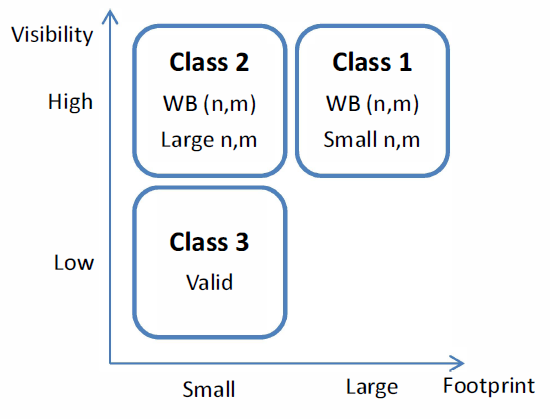
\includegraphics[width=\textwidth/2]{app_cat}
	\caption{Application categorization according to the cold row's policies \cite{refrint}.}
	\label{fig:app_cat}
\end{figure}

The technique modifies the MC. Which modifications and how large overhead? 5 bit snapshot for each row + state and n+m counters. some logic as well.

Presents the results. Add that we can not really use the result as they are from eDRAM.
